%%%%%%%%%%%%%%%%%%%%%%%%%%%%%%%%%%%%%%%%%%%%%%%%%%%%%%%%%%%%%%%%%%%%%%%%%%%%%%%

\section*{\large Exercício 5 - Processos Estocásticos Canônicos: Caos Determinístico e Turbulência}
\addcontentsline{toc}{chapter}{\protect\numberline{}\large Exercício 5}%

Os resultados deste exercício se encontram na pasta \textbf{Exercise4}, junto com todas as análises da família chaosnoise, separadas entre a pasta \textbf{Logístico} e \textbf{Henon}.

\subsection*{5.1}
\addcontentsline{toc}{section}{\protect\numberline{} 5.1}%

\subsubsection*{Logístico}
Para o mapeamento Logístico, os valores de $\rho$ escolhidos foram 3.81, 3.905 e 4. 

\begin{figure}[ht!]
	%\caption{Série e histogramas.}
	\vspace{0mm}	% acrescentar o espaçamento vertical apropriado entre o título e a borda superior da figura
	\begin{center}
		\resizebox{16cm}{!}{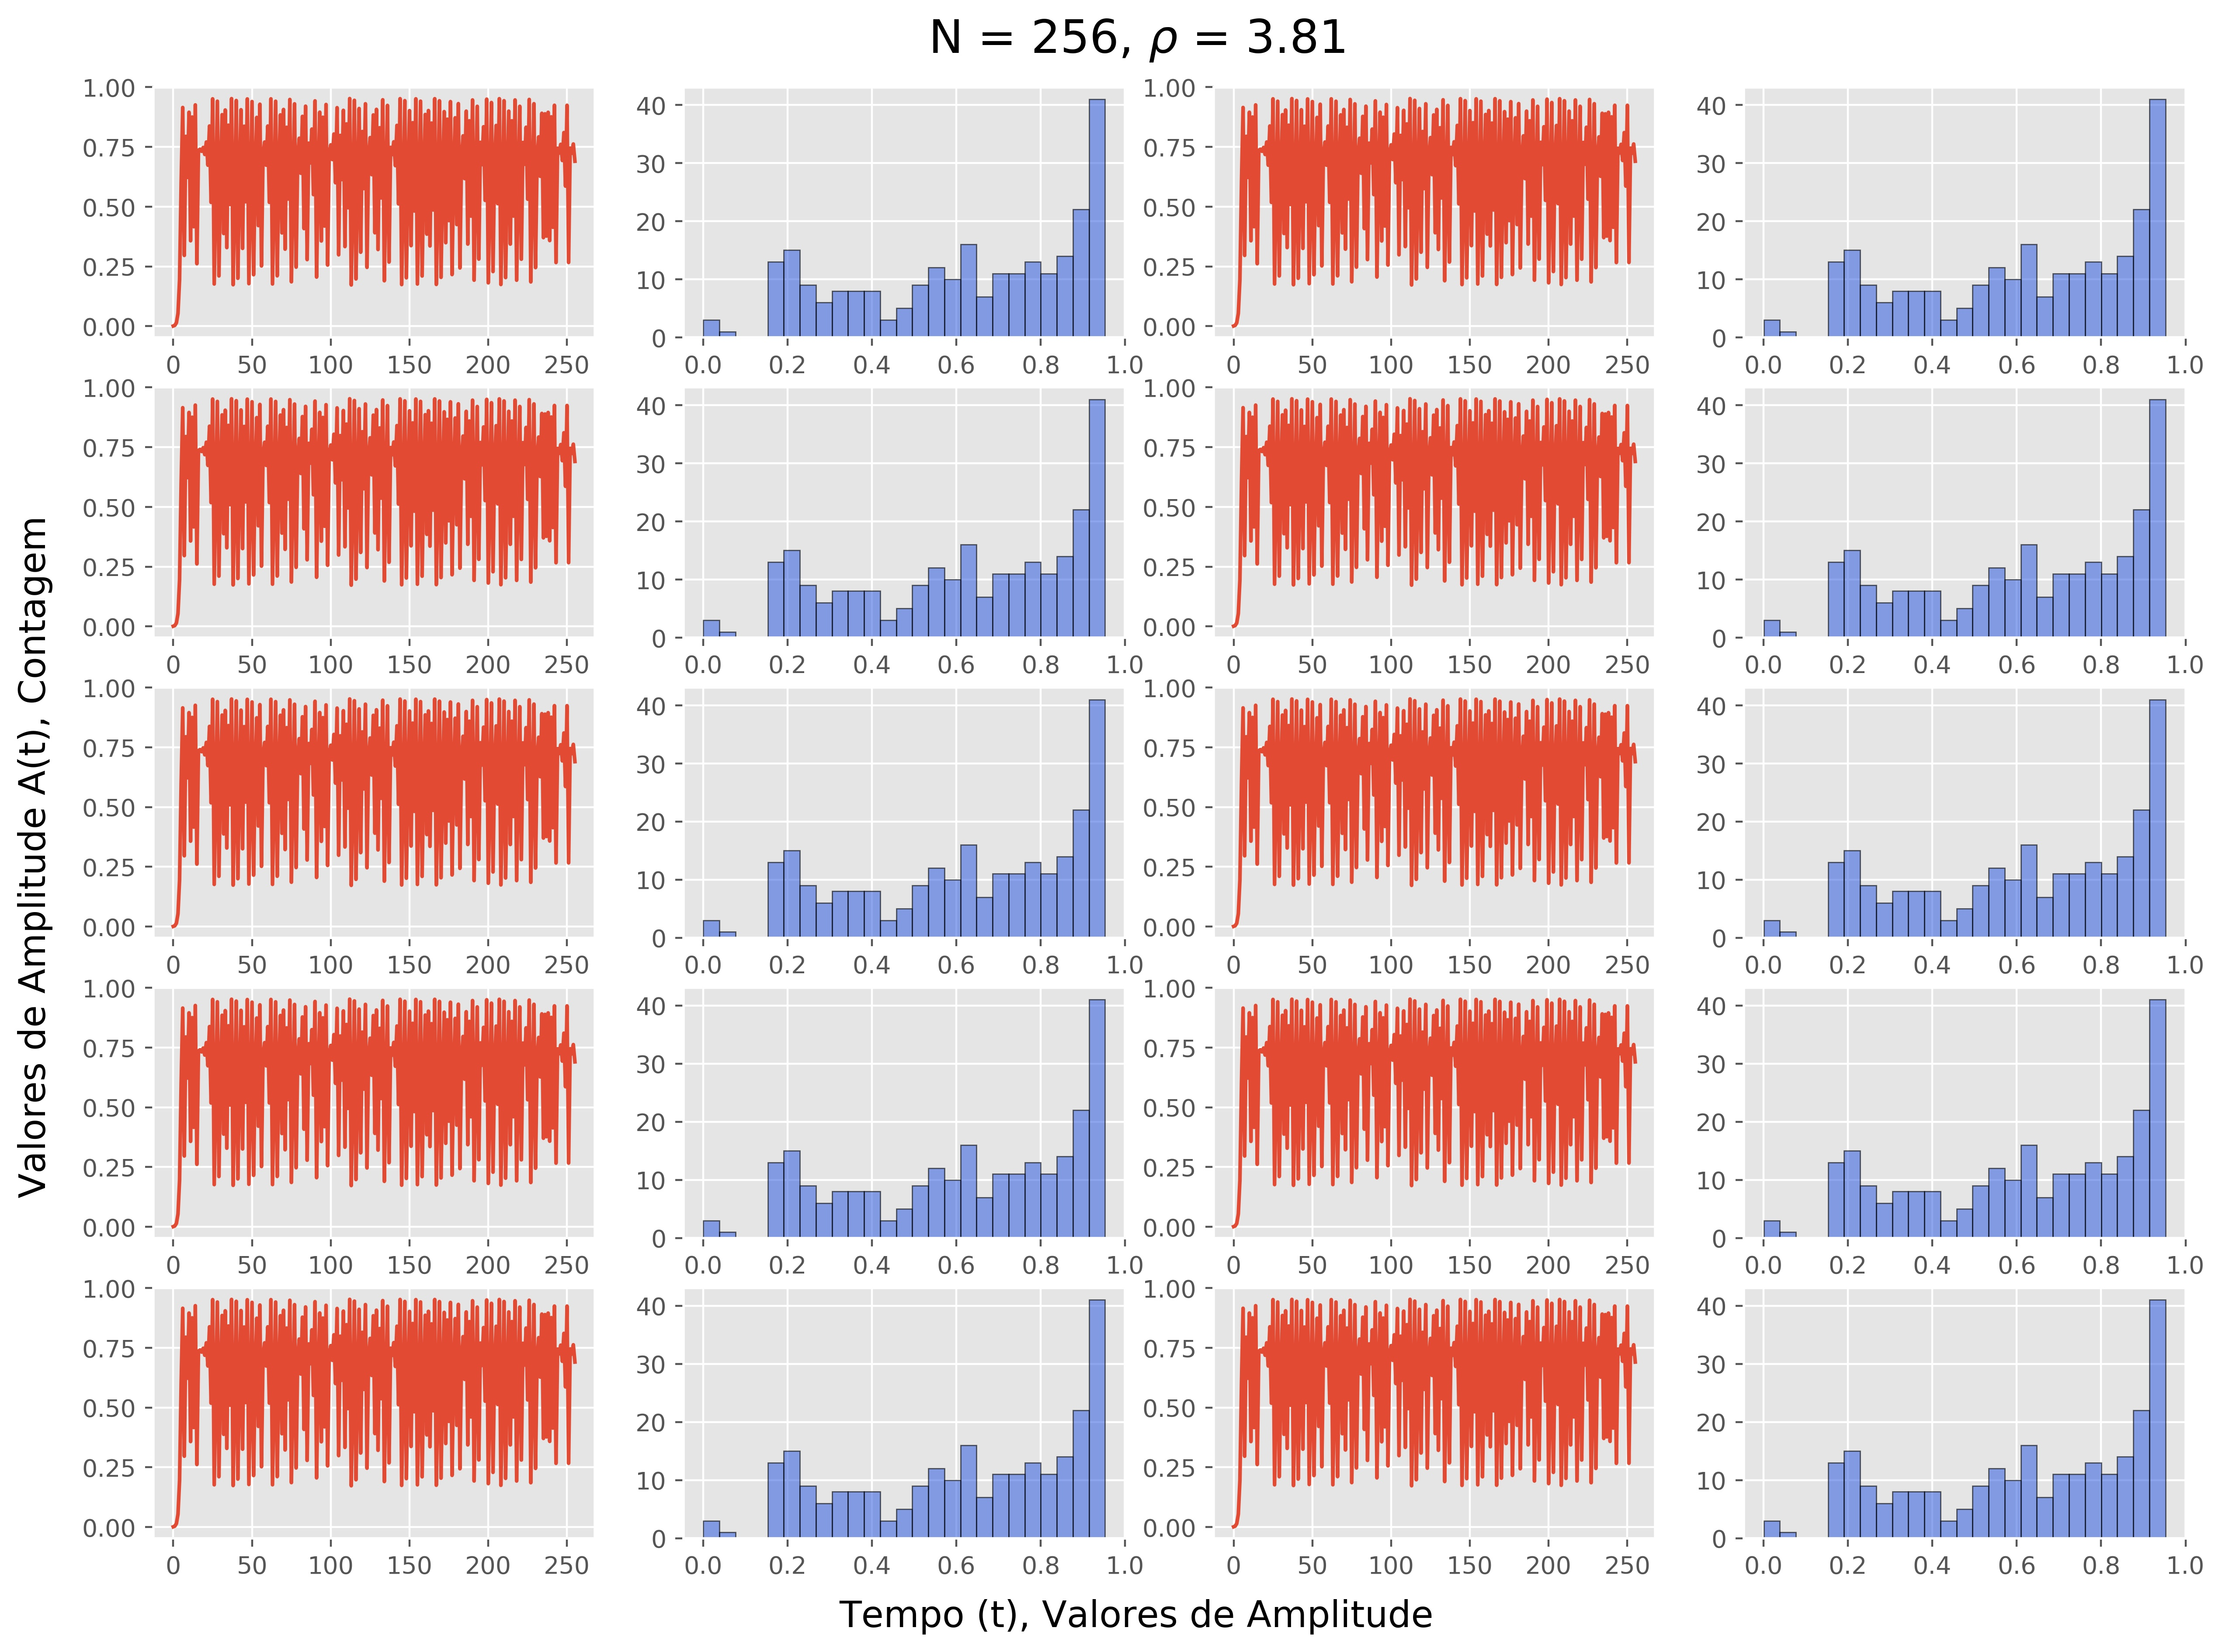
\includegraphics{Figuras/ex5/Logistico/Exercicio5_1_Logistico_n_256_rho_3.81.jpg}}		
	\end{center}
	\vspace{-2mm}	% acrescentar o espaçamento vertical apropriado entre a borda inferior da figura e a legenda ou a fonte quando não há legenda (o valor pode ser negativo para subir)
	\legenda{Figura 5.1.1: Plots de 10 sinais para a o mapeamento Logístico da família chaosnoise e seus respectivos histogramas. O tamanho da série foi de 256 para todos os valores de $\rho$. Acima os resultados para $\rho$ = 3.81.}	% legenda - para deixar sem legenda usar comando \legenda{} (nunca deve-se comentar o comando \legenda)
	\label{ex4_fig1}
	%\FONTE{}	% fonte consultada (elemento obrigatório, mesmo que seja produção do próprio autor)
\end{figure}

\clearpage
Os mesmos scripts da quarta questão foram implementados nas análises da família chaosnoise. A seguir são apresentados a classificação no espaço de Cullen and Frey e um ajuste de distribuições (incluindo GEV) a um dos sinais do mapeamento Logístico com $\rho$ = 3.81 (mais precisamente, o último sinal da Figura 5.1.1).

\begin{figure}[ht!]
	%\caption{Série e histogramas.}
	\vspace{0mm}	% acrescentar o espaçamento vertical apropriado entre o título e a borda superior da figura
	\begin{center}
		\resizebox{16cm}{!}{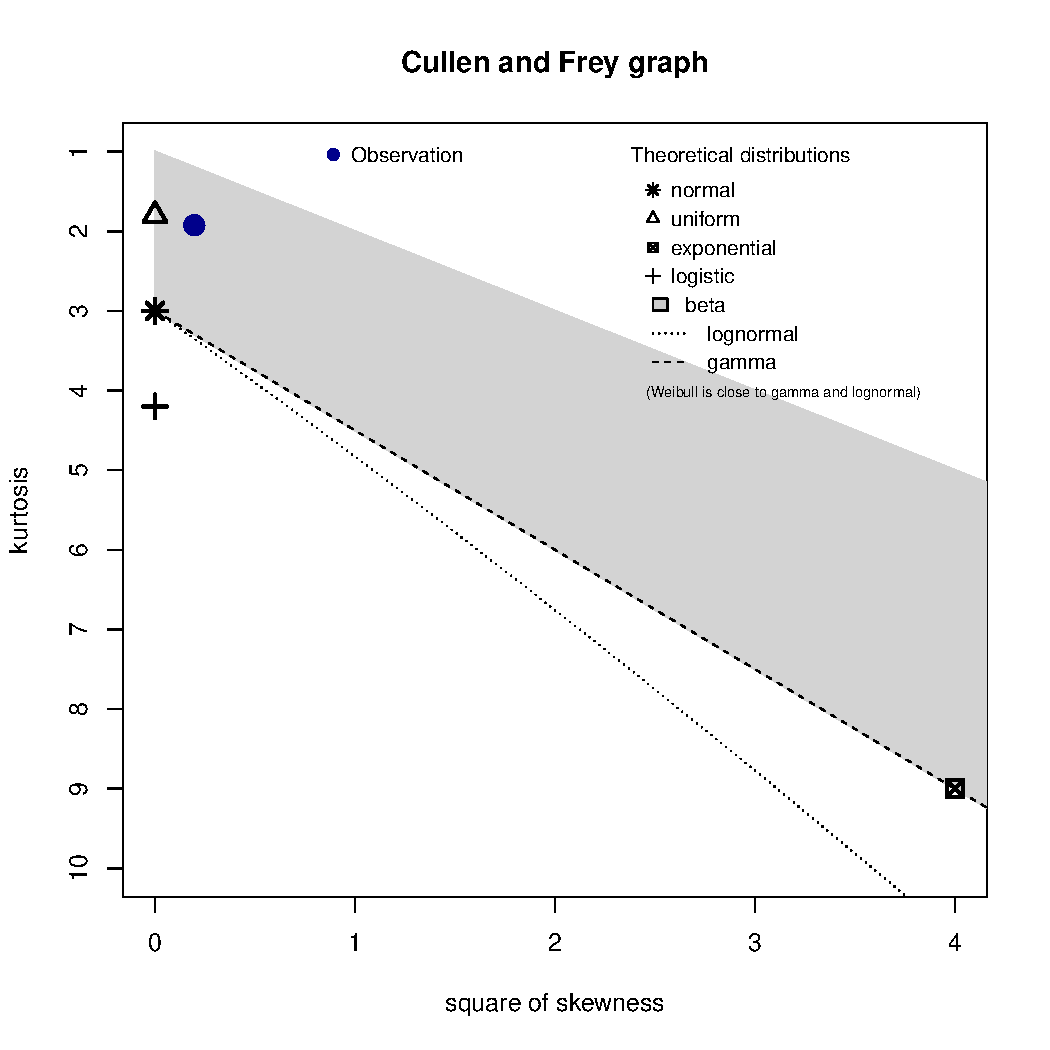
\includegraphics{Figuras/ex5/Logistico/rho_3.81_CullenFrey.pdf}}		
	\end{center}
	\vspace{-2mm}	% acrescentar o espaçamento vertical apropriado entre a borda inferior da figura e a legenda ou a fonte quando não há legenda (o valor pode ser negativo para subir)
	\legenda{Figura 5.1.2: Resultado da análise no espaço de Cullen and Frey para o mapeamento Logístico com $N$ = 256 e $\rho$ = 3.81 (último sinal da Figura 5.1.1).}	% legenda - para deixar sem legenda usar comando \legenda{} (nunca deve-se comentar o comando \legenda)
	\label{ex4_fig1}
	%\FONTE{}	% fonte consultada (elemento obrigatório, mesmo que seja produção do próprio autor)
\end{figure}

\clearpage

\begin{figure}[ht!]
	%\caption{Série e histogramas.}
	\vspace{0mm}	% acrescentar o espaçamento vertical apropriado entre o título e a borda superior da figura
	\begin{center}
		\resizebox{13cm}{!}{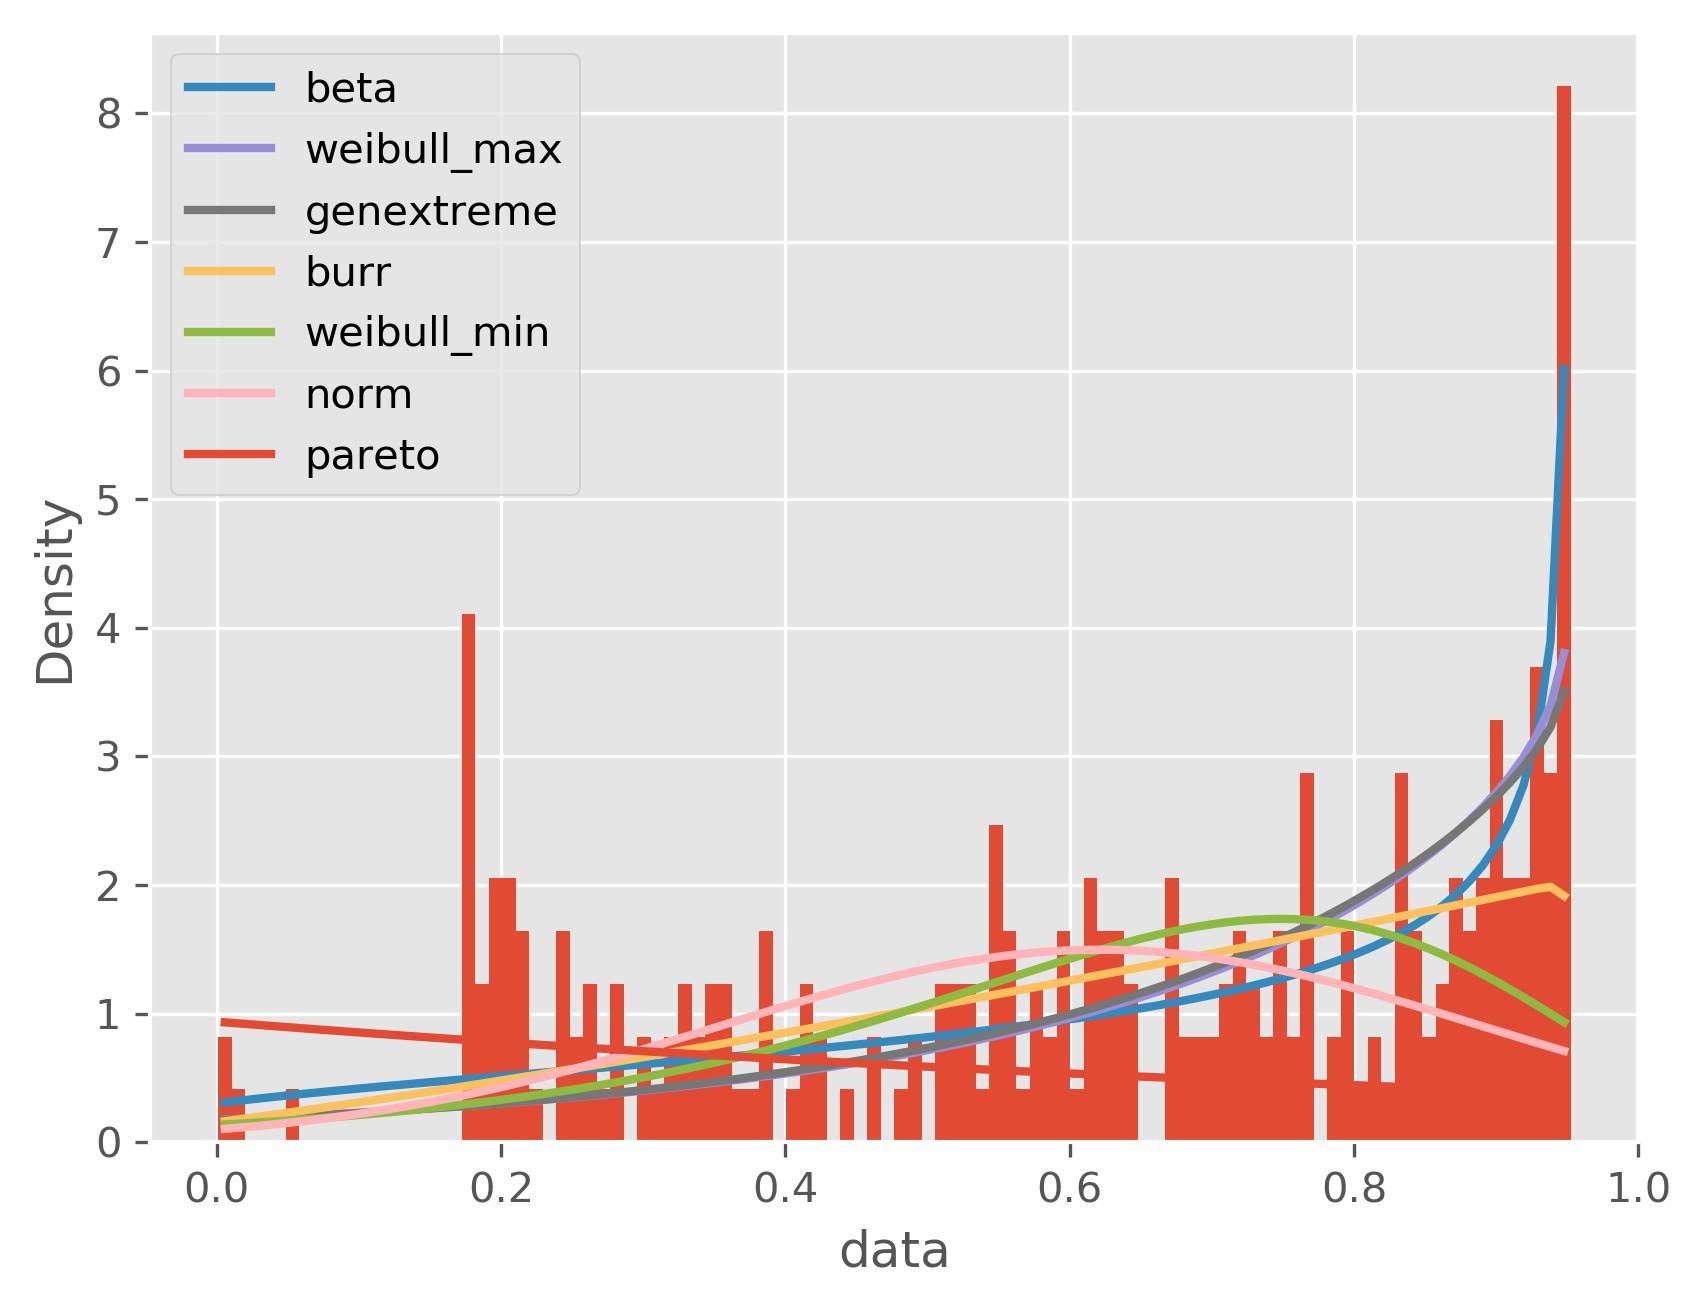
\includegraphics{Figuras/ex5/Logistico/rho_3.81_Python_fits.jpg}}		
	\end{center}
	\vspace{-2mm}	% acrescentar o espaçamento vertical apropriado entre a borda inferior da figura e a legenda ou a fonte quando não há legenda (o valor pode ser negativo para subir)
	\legenda{Figura 5.1.3: Resultado do ajuste de 7 distribuições ao último sinal presente na Figura 5.1.1.}	% legenda - para deixar sem legenda usar comando \legenda{} (nunca deve-se comentar o comando \legenda)
	\label{ex4_fig1}
	%\FONTE{}	% fonte consultada (elemento obrigatório, mesmo que seja produção do próprio autor)
\end{figure}

Resultado do benchmark do ajuste das distribuições. Observa-se que a distribuição \texttt{beta} foi a de melhor ajuste. Esse resultado se encontra no arquivo \textit{rho\_3.81\_Python\_fits.txt}.

\begin{figure}[ht!]
	%\caption{Série e histogramas.}
	\vspace{0mm}	% acrescentar o espaçamento vertical apropriado entre o título e a borda superior da figura
	%\begin{center}
		\resizebox{13cm}{!}{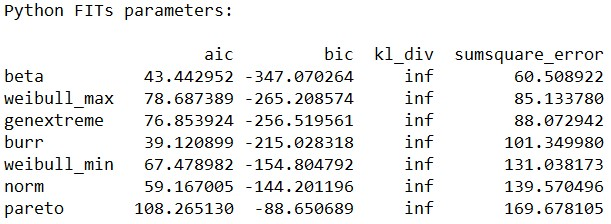
\includegraphics{Figuras/ex5/Logistico/rho_3.81_Python_fits_params.jpg}}		
	%\end{center}
	\vspace{-2mm}	% acrescentar o espaçamento vertical apropriado entre a borda inferior da figura e a legenda ou a fonte quando não há legenda (o valor pode ser negativo para subir)
	%\legenda{Figura 5.3:.}	% legenda - para deixar sem legenda usar comando \legenda{} (nunca deve-se comentar o comando \legenda)
	\label{ex4_fig1}
	%\FONTE{}	% fonte consultada (elemento obrigatório, mesmo que seja produção do próprio autor)
\end{figure}

%%%%%%%%%%%%%%%%%%%%%%%%%%%%%%%%%%% Henon %%%%%%%%%%%%%%%%%%%%%%%%%%%%%%%%%%%%%%%%%%

\clearpage
\subsubsection*{Henon}
Para o mapeamento de Henon, os valores de $a$ escolhidos foram 1.32 e 1.4. Para $b$, escolheu-se os valores 0.21, 0.26 e 0.31, de forma a fixar o primeiro e variar o segundo gerando-se cinco sinais para cada combinação de parâmetros.


\begin{figure}[ht!]
  \begin{adjustbox}{addcode={\begin{minipage}{\width}}{\\% 
      Figura 5.1.4: Série de 15 sinais diferentes (e seus respectivos histogramas) gerados com o script chaosnoise.py. A figura exibe o resultado de $a$ = 1.32 e três valores de $b$. Os cinco primeiros sinais (da esquerda) são para $b$ = 0.21, os cinco do centro para $b$ = 0.26, e os cinco da direita para $b$ = 0.31.
      \end{minipage}},rotate=90,center}
      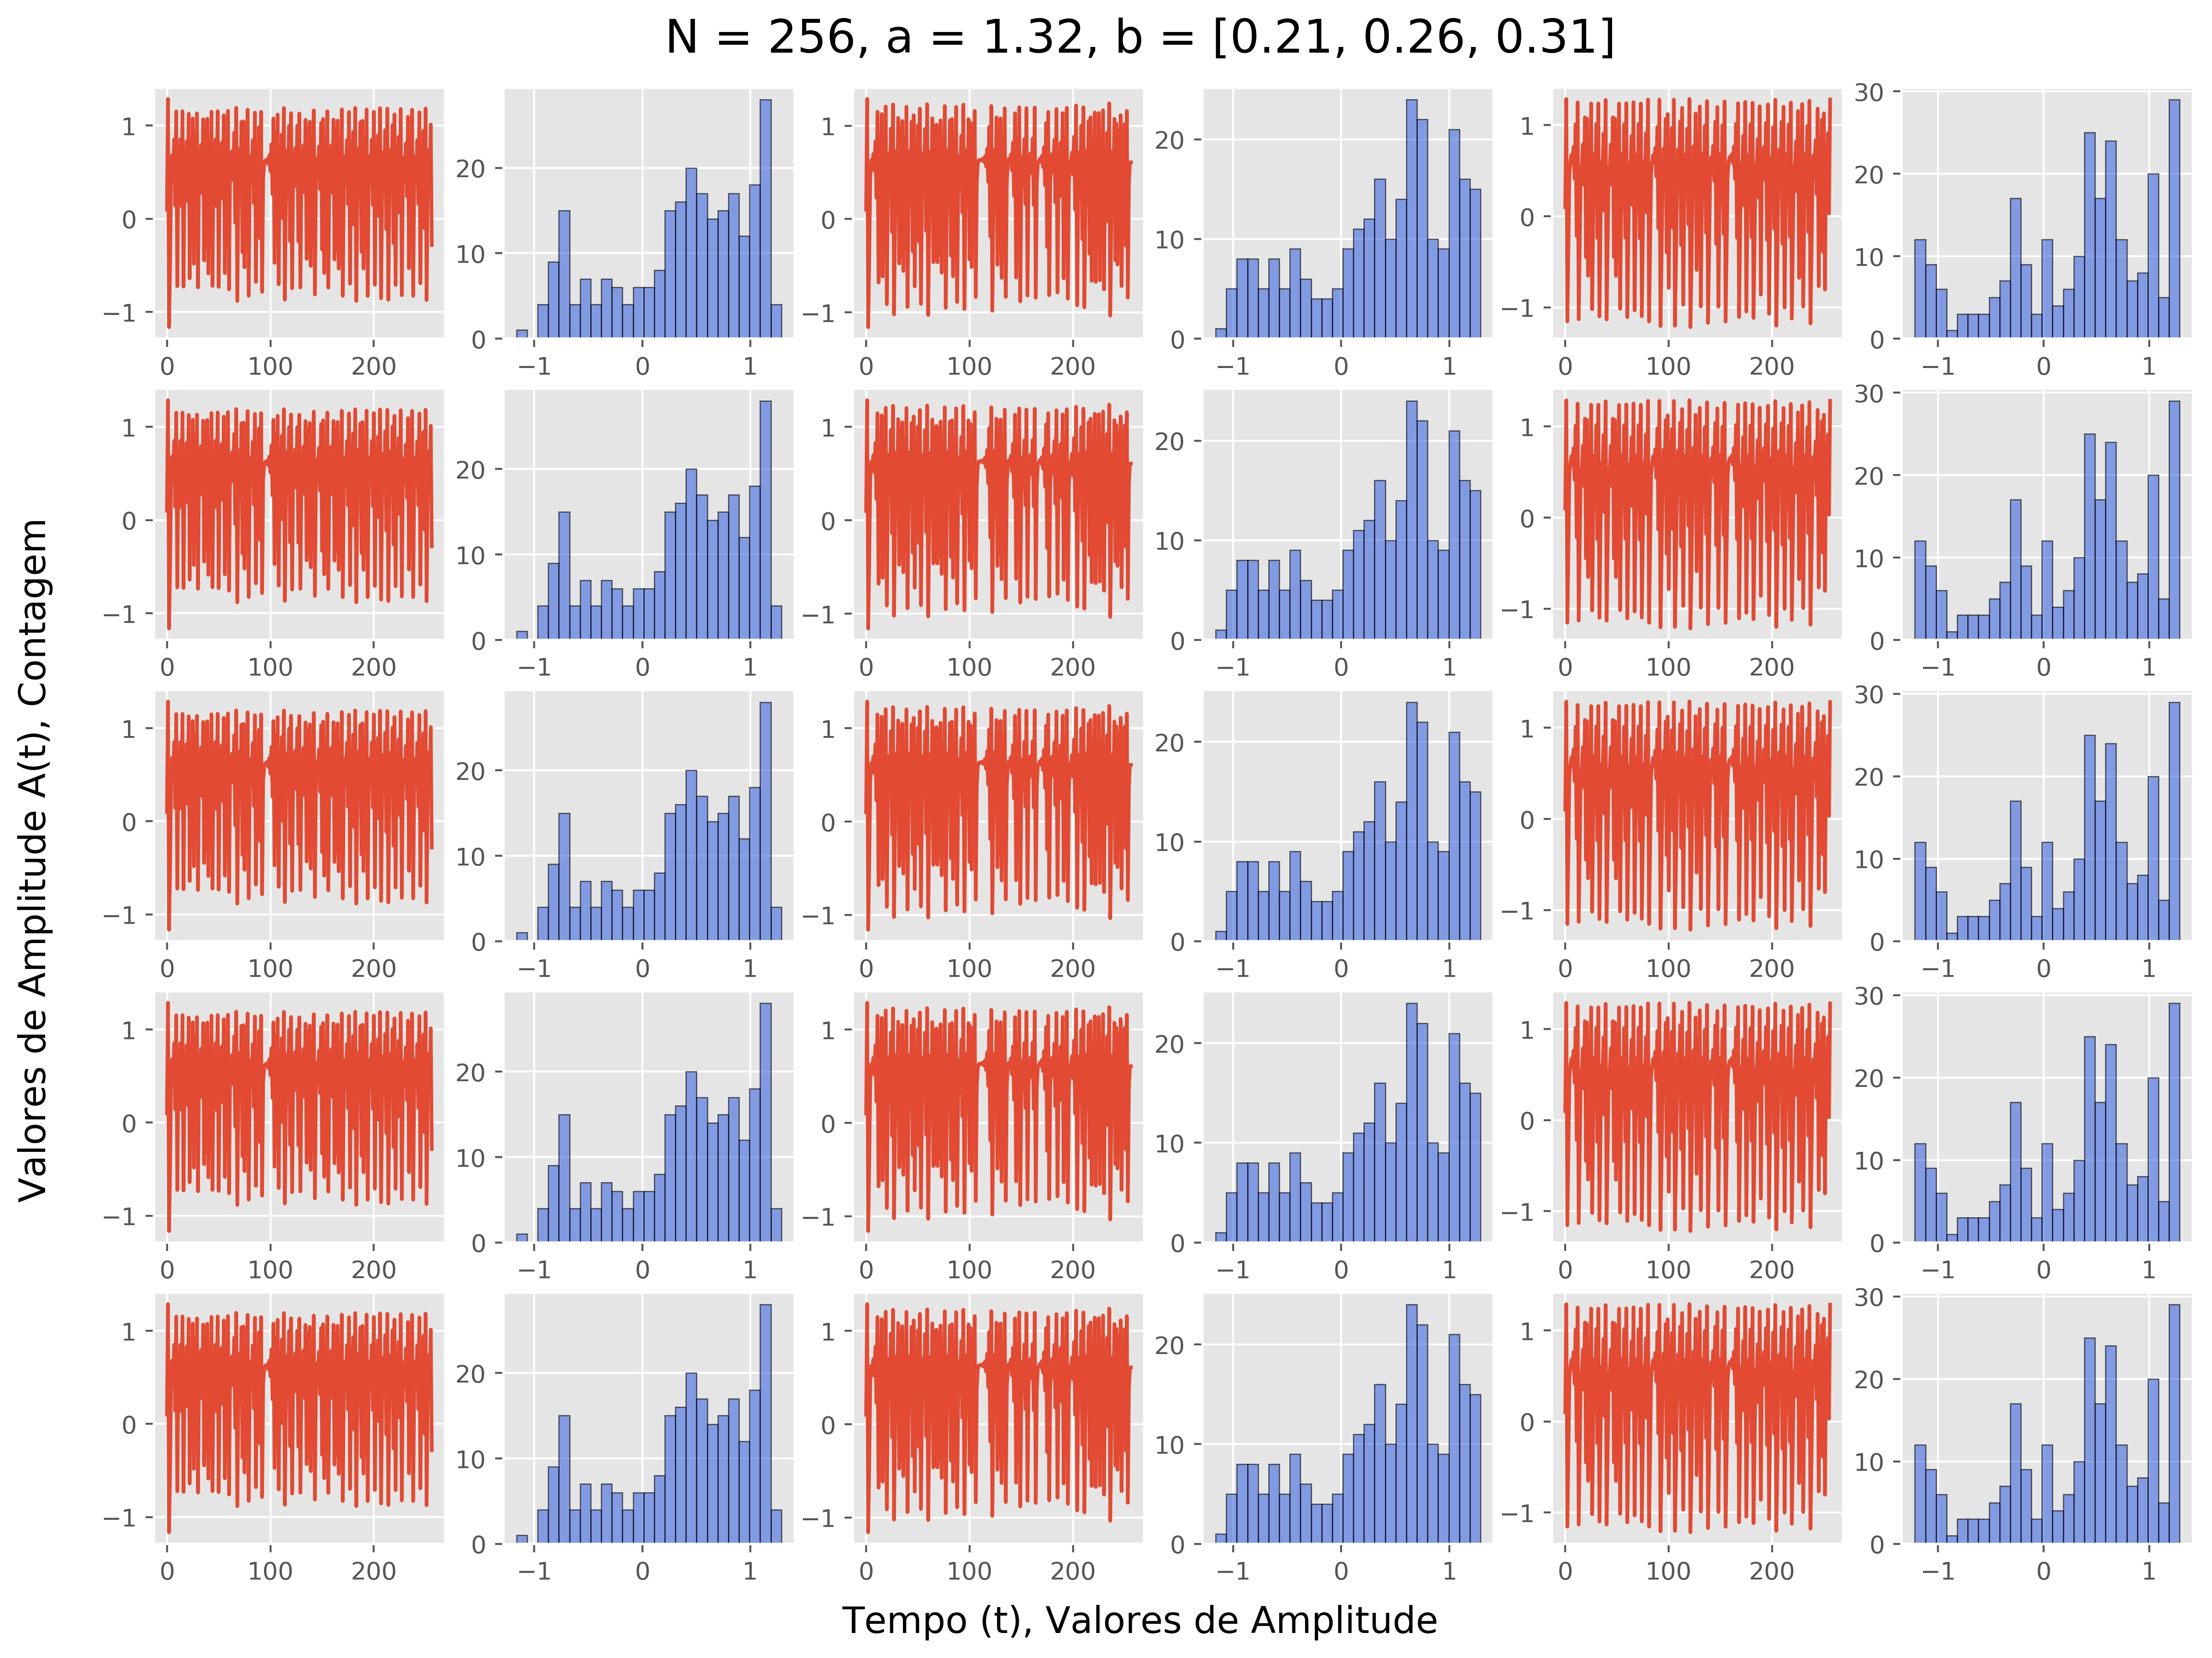
\includegraphics[scale=.5]{Figuras/ex5/Henon/Exercicio5_1_Henon_n_256_a_1.32.jpg}	%
  \end{adjustbox}
\end{figure}

%\begin{figure}[ht!]
%	%\caption{Série e histogramas.}
%	\vspace{0mm}	% acrescentar o espaçamento vertical apropriado entre o título e a borda superior da figura
%	\begin{center}
%		\resizebox{17cm}{!}{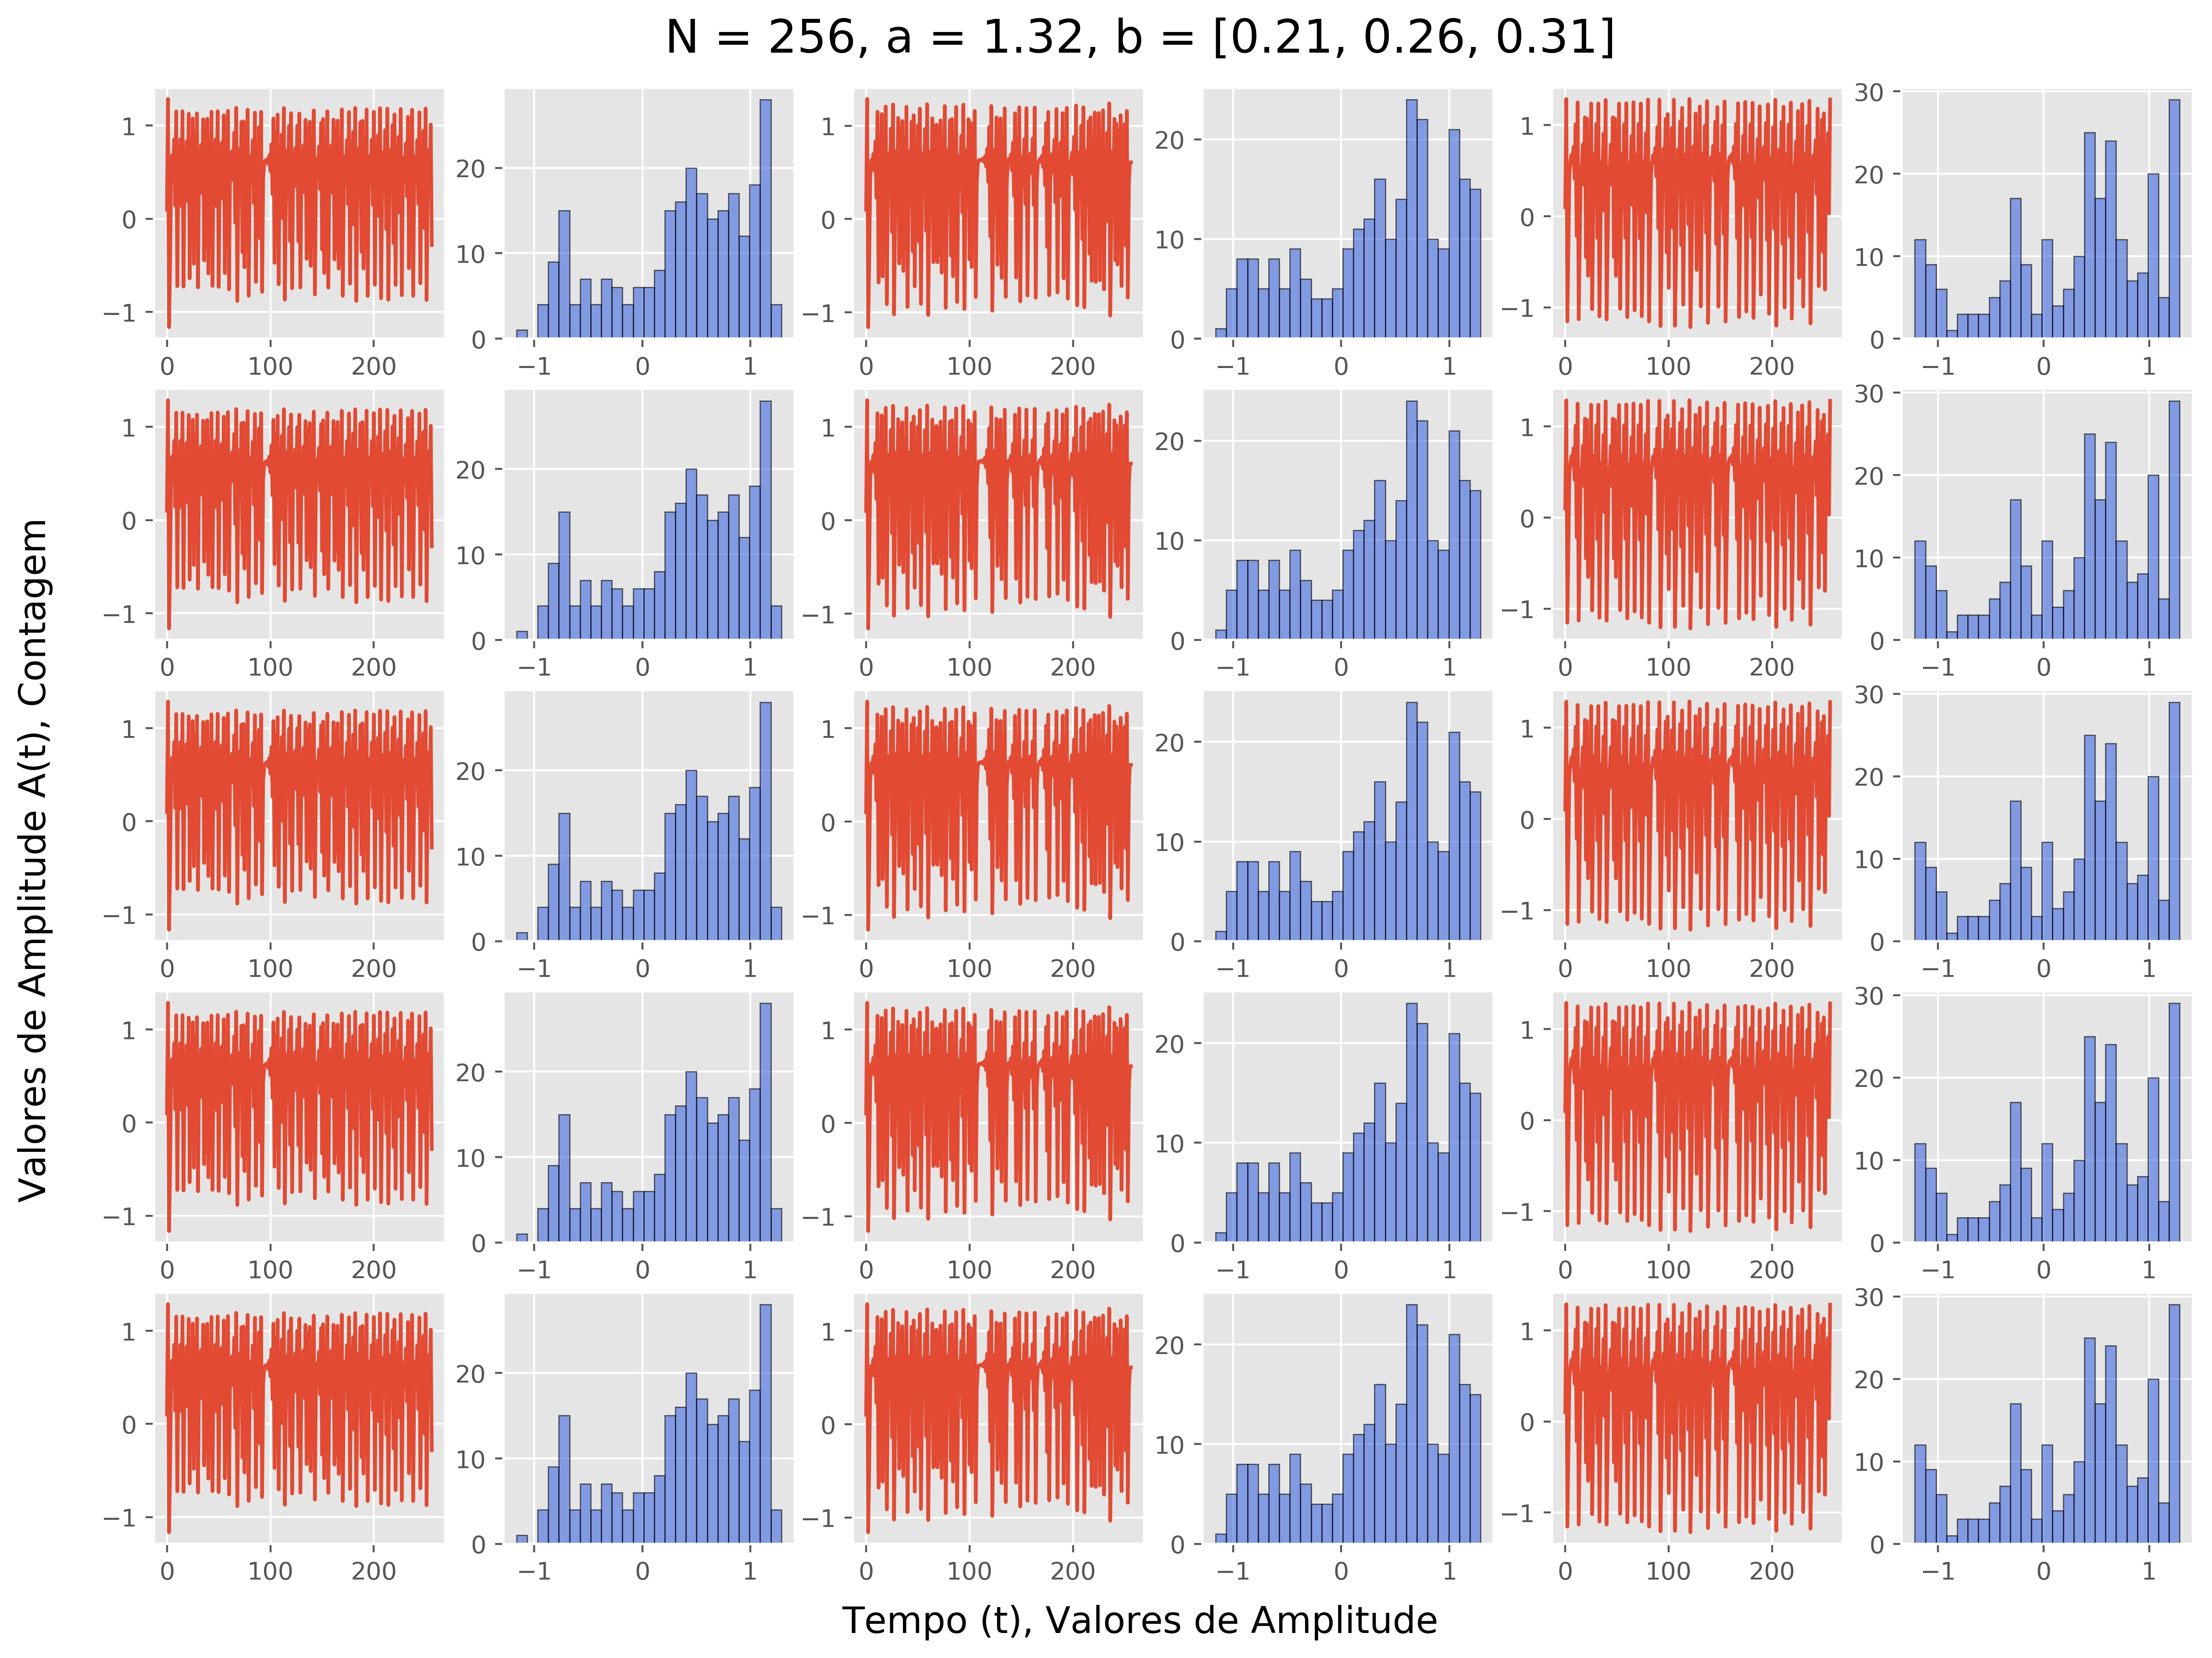
\includegraphics{Figuras/ex5/Henon/Exercicio5_1_Henon_n_256_a_1.32.jpg}}		
%	\end{center}
%	\vspace{-2mm}	% acrescentar o espaçamento vertical apropriado entre a borda inferior da figura e a legenda ou a fonte quando não há legenda (o valor pode ser negativo para subir)
%	\legenda{Figura 5.1.4:.}	% legenda - para deixar sem legenda usar comando \legenda{} (nunca deve-se comentar o comando \legenda)
%	\label{ex4_fig1}
	%\FONTE{}	% fonte consultada (elemento obrigatório, mesmo que seja produção do próprio autor)
%\end{figure}

A seguir são apresentados a classificação no espaço de Cullen and Frey e um ajuste de distribuições (incluindo GEV) a um dos sinais do mapeamento de Henon com $a$ = 1.32 e $b$ = 0.31 (mais precisamente, o último sinal da Figura 5.1.4).

\begin{figure}[ht!]
	%\caption{Série e histogramas.}
	\vspace{0mm}	% acrescentar o espaçamento vertical apropriado entre o título e a borda superior da figura
	\begin{center}
		\resizebox{16cm}{!}{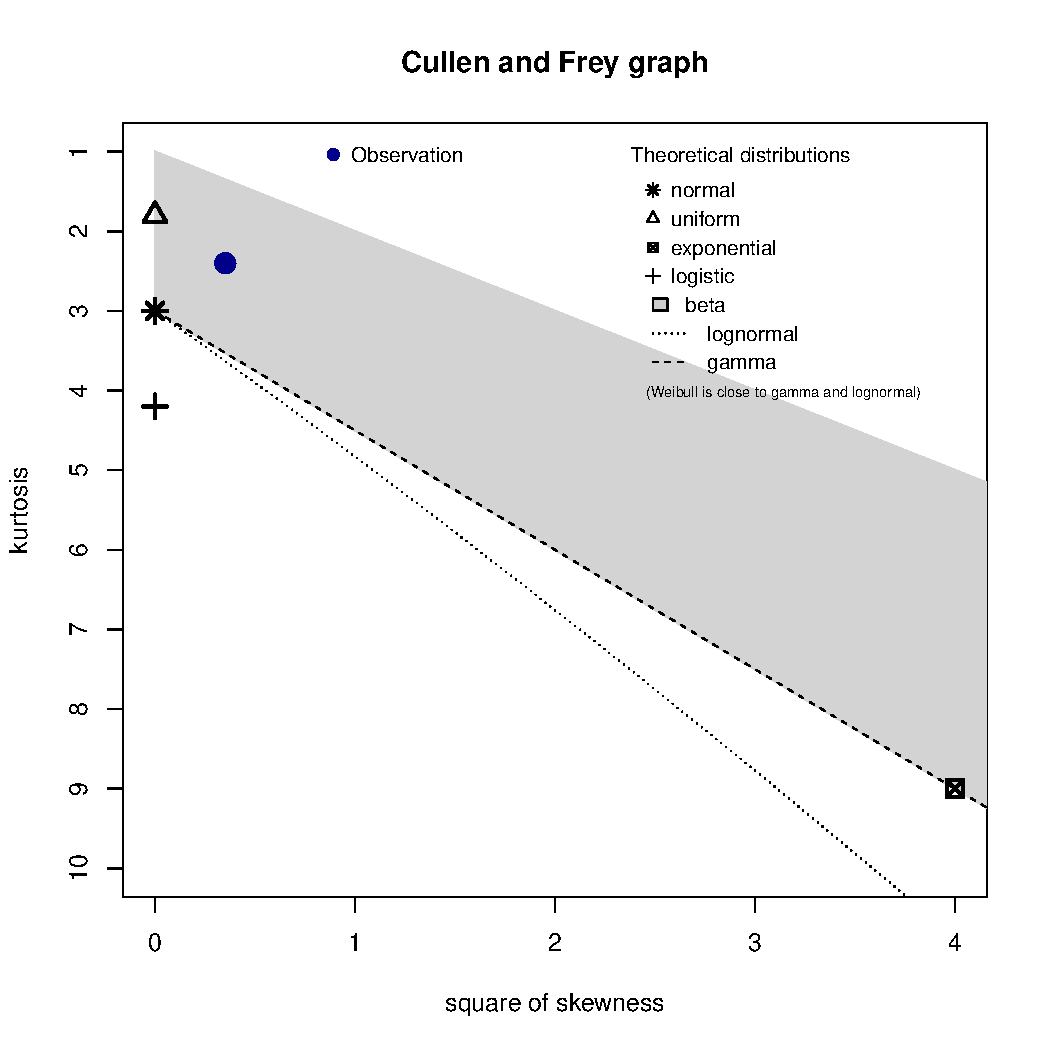
\includegraphics{Figuras/ex5/Henon/a_1.32_b_0.31_CullenFrey.pdf}}		
	\end{center}
	\vspace{-2mm}	% acrescentar o espaçamento vertical apropriado entre a borda inferior da figura e a legenda ou a fonte quando não há legenda (o valor pode ser negativo para subir)
	\legenda{Figura 5.1.5: Resultado da análise no espaço de Cullen and Frey para o mapeamento de Henon com $a$ = 1.32 e $b$ = 0.31 (último sinal da Figura 5.1.4).}	% legenda - para deixar sem legenda usar comando \legenda{} (nunca deve-se comentar o comando \legenda)
	\label{ex4_fig1}
	%\FONTE{}	% fonte consultada (elemento obrigatório, mesmo que seja produção do próprio autor)
\end{figure}

\clearpage 

\begin{figure}[ht!]
	%\caption{Série e histogramas.}
	\vspace{0mm}	% acrescentar o espaçamento vertical apropriado entre o título e a borda superior da figura
	\begin{center}
		\resizebox{13cm}{!}{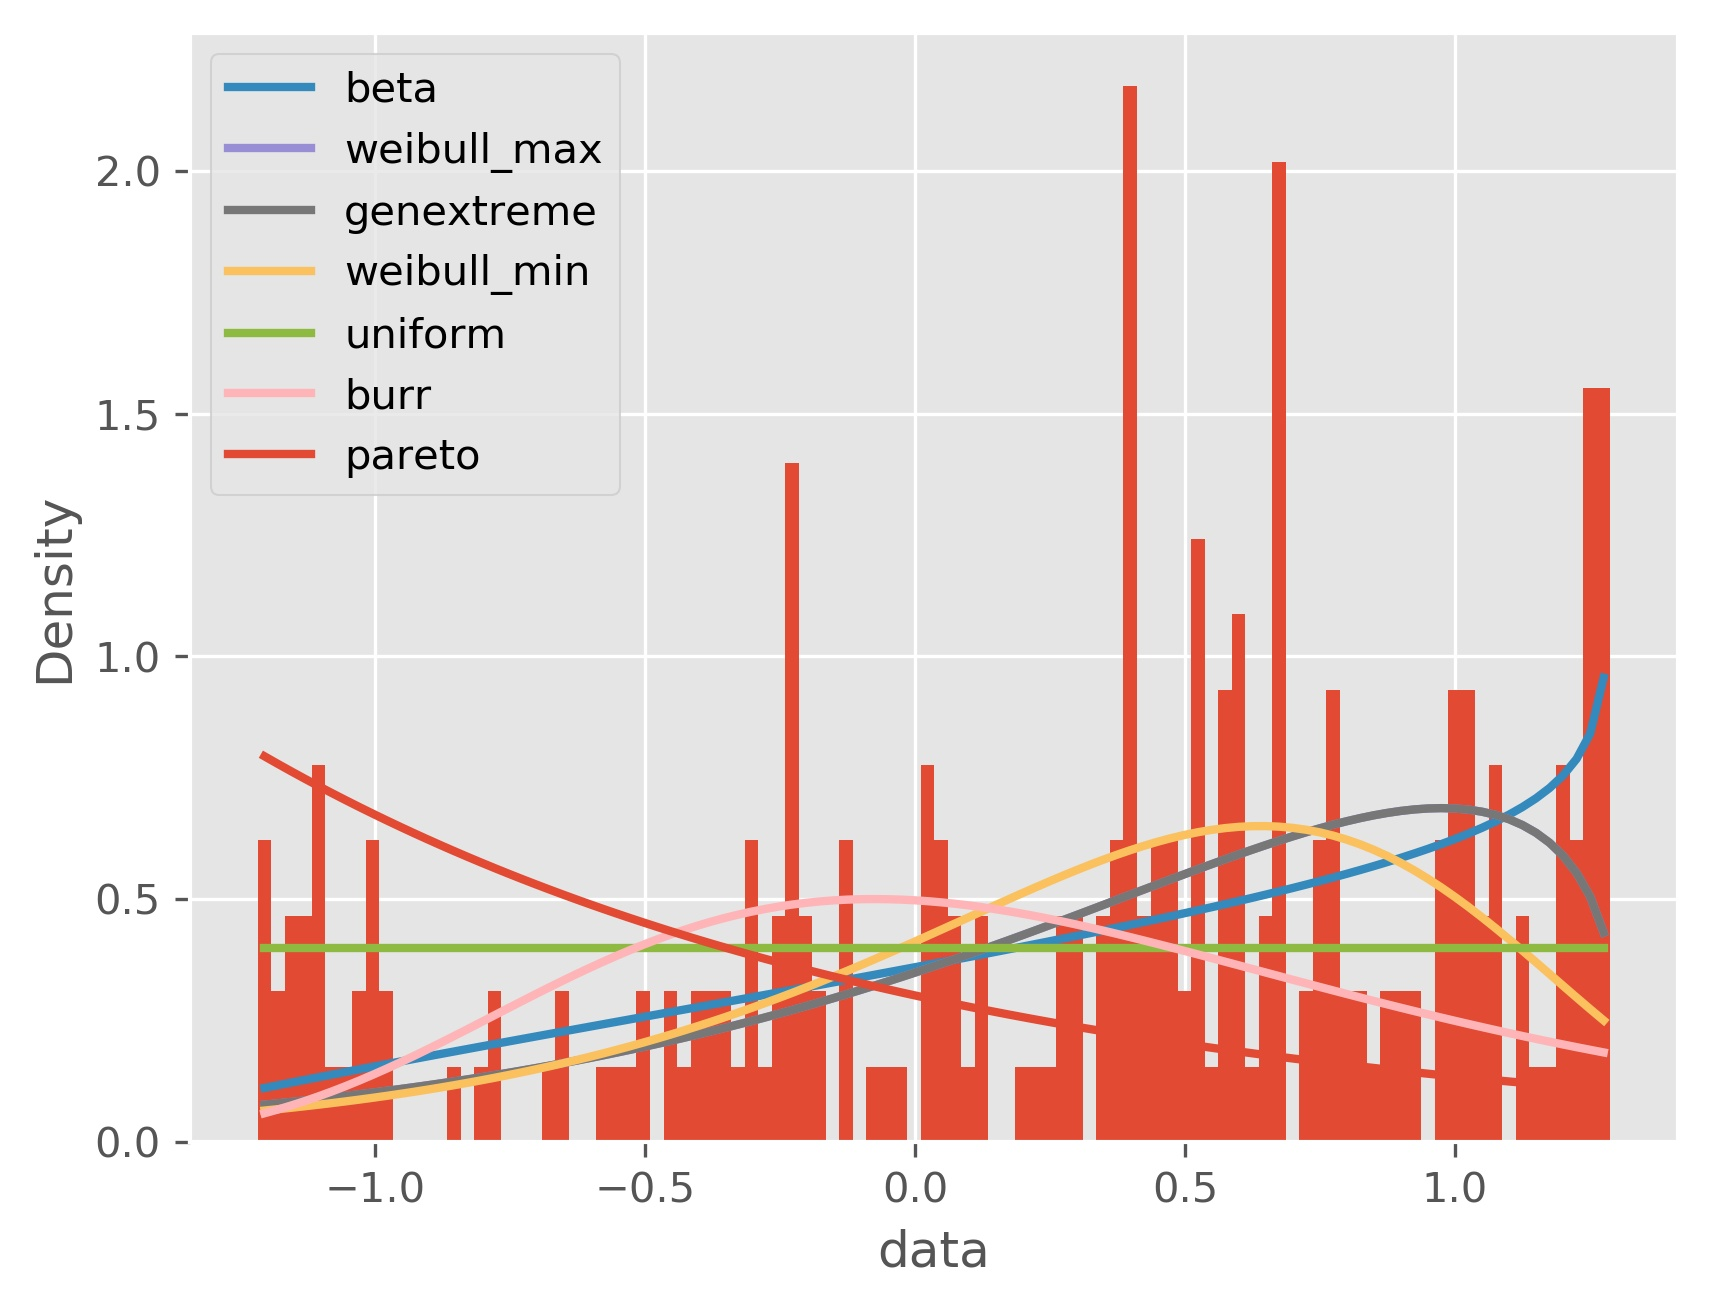
\includegraphics{Figuras/ex5/Henon/a_1.32_b_0.31_Python_fits.jpg}}		
	\end{center}
	\vspace{-2mm}	% acrescentar o espaçamento vertical apropriado entre a borda inferior da figura e a legenda ou a fonte quando não há legenda (o valor pode ser negativo para subir)
	\legenda{Figura 5.1.6: Resultado do ajuste de 7 distribuições ao último sinal presente na Figura 5.1.4.}	% legenda - para deixar sem legenda usar comando \legenda{} (nunca deve-se comentar o comando \legenda)
	\label{ex4_fig1}
	%\FONTE{}	% fonte consultada (elemento obrigatório, mesmo que seja produção do próprio autor)
\end{figure}

Resultado do benchmark do ajuste das distribuições. Novamente, observa-se que a distribuição \texttt{beta} foi a de melhor ajuste. Esse resultado se encontra no arquivo \textit{a\_1.32\_b\_0.31\_Python\_fits.txt}.

\begin{figure}[ht!]
	%\caption{Série e histogramas.}
	\vspace{0mm}	% acrescentar o espaçamento vertical apropriado entre o título e a borda superior da figura
	%\begin{center}
		\resizebox{13cm}{!}{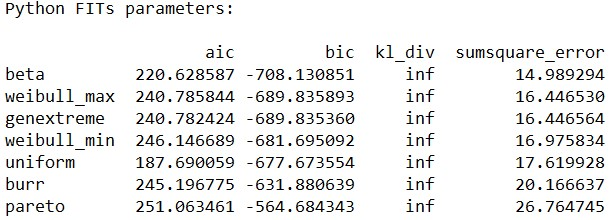
\includegraphics{Figuras/ex5/Henon/a_1.32_b_0.31_Python_fits_params.jpg}}		
	%\end{center}
	\vspace{-2mm}	% acrescentar o espaçamento vertical apropriado entre a borda inferior da figura e a legenda ou a fonte quando não há legenda (o valor pode ser negativo para subir)
	%\legenda{Figura 5.3:.}	% legenda - para deixar sem legenda usar comando \legenda{} (nunca deve-se comentar o comando \legenda)
	\label{ex4_fig1}
	%\FONTE{}	% fonte consultada (elemento obrigatório, mesmo que seja produção do próprio autor)
\end{figure}

%%%%%%%%%%%%%%%%%%%%%%%%%%%%%%%%%%%%%%%%% 5.2 %%%%%%%%%%%%%%%%%%%%%%%%%%%%%%%%%%%%%%%%%%

\clearpage
\subsection*{5.2}
\addcontentsline{toc}{section}{\protect\numberline{} 5.2}%

A segunda lei de Newton é definida por:

\begin{equation*}
\sum\vec{f}_{ext} = m \vec{a},
\end{equation*}

que representa que a aceleração de um corpor é devido ao somatório das forças externas aplicadas à ele. Para uma parcela de fluido de densidade $\rho$, a força por unidade de volume é

\begin{equation*}
\sum\vec{f} = \rho \vec{a} = \vec{f}_{grav} + \vec{f}_{press} + \vec{f}_{visc},
\end{equation*}

onde $\vec{f}_{grav}$ = $\rho\vec{g}$ é a força gravitacional, agindo sobre o fluido na direção negativa de $\vec{z}$, ou seja, para baixo; $\vec{f}_{press}$ = $-\vec{\nabla}p$ representa as forças de pressão, agindo sobre o fluido em todas as direções, para o seu interior e normal à sua superfície; $\vec{f}_{visc}$ = $\mu \nabla^{2} \vec{v}$ denota a força viscosa, que 
é proporcional à velocidade $v$ do fluido e age em sua superfície (normalmente ou tangencialmente) por conta da viscosidade $\mu$ do mesmo ($\nabla^{2}$ é o operador Laplaciano).

Expandindo a aceleração, escrevendo-a em termos de derivadas dos componentes da velocidade, e substituindo cada um dos componentes de força atuando sobre a parcela de fluido, temos

\begin{equation*}
\rho \left( \frac{\partial \vec{v}}{\partial t} + \vec{v}_{x}\frac{\partial \vec{v}}{\partial x} + \vec{v}_{y}\frac{\partial \vec{v}}{\partial y} + \vec{v}_{z}\frac{\partial \vec{v}}{\partial z} \right) = \rho\vec{g} - \vec{\nabla}p + \mu \nabla^{2} \vec{v},
\end{equation*}

que é a equação de \textit{Navier-Stokes} válida para fluidos Newtonianos incompressíveis. 